\let\negmedspace\undefined
\let\negthickspace\undefined
\documentclass[journal]{IEEEtran}
\usepackage[a5paper, margin=10mm, onecolumn]{geometry}
\usepackage{lmodern} % Ensure lmodern is loaded for pdflatex
\usepackage{tfrupee} % Include tfrupee package

\setlength{\headheight}{1cm} % Set the height of the header box
\setlength{\headsep}{0mm}     % Set the distance between the header box and the top of the text

\usepackage{gvv-book}
\usepackage{gvv}
\usepackage{cite}
\usepackage{amsmath,amssymb,amsfonts,amsthm}
\usepackage{algorithmic}
\usepackage{graphicx}
\usepackage{textcomp}
\usepackage{xcolor}
\usepackage{txfonts}
\usepackage{listings}
\usepackage{enumitem}
\usepackage{mathtools}
\usepackage{gensymb}
\usepackage{comment}
\usepackage[breaklinks=true]{hyperref}
\usepackage{tkz-euclide} 
\usepackage{listings}
\usepackage{gvv}                                        
\def\inputGnumericTable{}                                 
\usepackage[latin1]{inputenc}                                
\usepackage{color}                                            
\usepackage{array}                                            
\usepackage{longtable}                                       
\usepackage{calc}                                             
\usepackage{multirow}                                         
\usepackage{hhline}                                           
\usepackage{ifthen}                                           
\usepackage{lscape}
\begin{document}

\bibliographystyle{IEEEtran}
\vspace{3cm}

\title{1-1.5-11}
\author{AI24BTECH11015 - Harshvardhan Patidar}
% \maketitle
% \newpage
% \bigskip
{\let\newpage\relax\maketitle}

\renewcommand{\thefigure}{\theenumi}
\renewcommand{\thetable}{\theenumi}
\setlength{\intextsep}{10pt} % Space between text and floats


\numberwithin{equation}{enumi}
\numberwithin{figure}{enumi}
\renewcommand{\thetable}{\theenumi}


	Question:\\
		The point $\vec{R}$ divides the line segment $AB$, where $\vec{A} \brak{-4,0} \text{and } \vec{B} \brak{0,6}$ such that $AR = \frac{3}{4}AB$. Find the coordinates of $\vec{R}$.
	\\
	\\
	\solution:\\

	We have,
	\begin{align}
		AR = \frac{3}{4} AB\\
		AR:RB = 3:1
	\end{align}

	We have, if $\vec{R}$ divides the line $AB$ in ratio $k:1$ then, $$\vec{R} = \brak{\frac{k\vec{B} + \vec{A}}{k+1}}$$.

	Using the above formula, the desired point is

	\begin{align}
		\frac{1}{3+1}\brak{3\myvec{0\\6} + \myvec{-4\\0}} \\
		\vec{R}=\myvec{-1\\4.5}
	\end{align}


	\begin{figure}[hbt!]
		\centering
		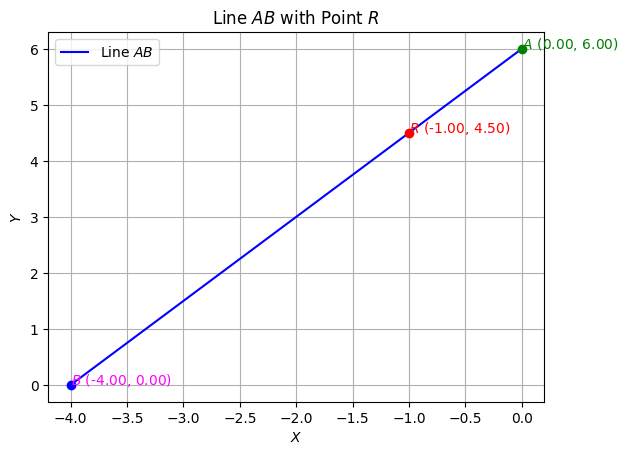
\includegraphics[width=0.6\linewidth]{plots/plot.png}

	\end{figure}

\end{document}


